\section{Partie Financière}

Lors du projet Activ'ESAIP, l'équipe d'étudiant vient se substituer à une équipe d'ingénieurs de conseil. C'est un dispositif intéressant pour l'entreprise car bien moins coûteux !\\

Il est intéressant d'estimer les gains réalisés par l'entreprise en choisissant le dispositif Activ'ESAIP, et c'est ce que nous allons estimer au cours de cette partie financière.

\subsection{Coût de l'Activ'ESAIP pour l'entreprise}

Lors de cette mission, trois étudiants ingénieurs ont été mobilisés par Panorama Performance : deux étudiants en Informatique et Réseaux et un étudiant en Sécurité, Environnement et Prévention des risques. Selon la grille tarifaire de l'ESAIP\footnote{Voir Annexe A}, cela correspond à une facture de 2550\euro. Cette somme est \textbf{TTC} car Panorama Performance ne récupère pas de \textbf{TVA}.\\

L'entreprise n'a pas eu de frais de déplacement supplémentaire à payer, car nous résidons tous les trois sur Angers. Bien que M. \textsc{Lecointre} soit légalement notre tuteur entreprise, c'est Mme. \textsc{Oudard} qui s'est chargée de nous encadrer et de répondre à nos questions en cas d'interrogations. Pour autant, nous avons su faire preuve d'autonomie sur une grande majorité du projet, ce qui a permis à l'équipe de Panorama Performance d'éviter des coûts indirects en consacrant du temps, normalement réservé à leurs clients, à ce projet. 

\subsection{Estimation des coûts réels de la mission}

Pour rappel, nous avons décidé de diviser nos 5 semaines en : 
\begin{itemize}
    \item Une semaine de recherche
    \item 3 semaines de développement et de rédaction d'un business model
    \item Une semaine de bilan entreprise et soutenance
\end{itemize}
L'équipe de Panorama Performance ne possédant pas de profil \textbf{IT}, il y aurait donc eu une obligation de faire appel à un tiers. Nous avons donc décidé de faire plusieurs hypothèses en appliquant les tarifs \textbf{free-lance} disponibles en lignes \cite{SalaireFreeLance}. Nos calculs sont basés sur une semaine d'étude de faisabilité et 3 semaines de développement (la $5^{e}$ n'est pas comptée car pas immédiatement reliée au projet).\\

En prenant un salaire moyen journalier de 500\euro/jour pour le développement de l'application, et de 400\euro/jour pour l'étude de faisabilité du projet, nous avons estimé un coût total pour le projet de 25.334\euro~HT.
\clearpage

\begin{figure}[!h]
    \centering
    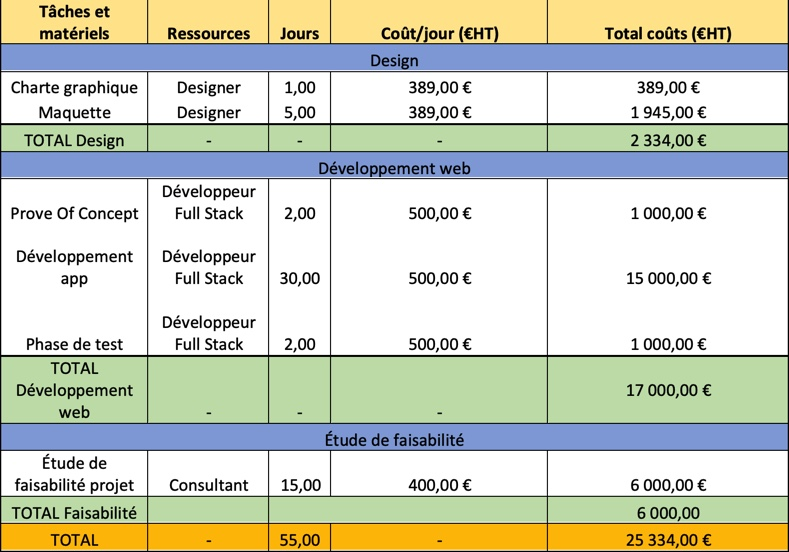
\includegraphics[scale=0.5]{img/estimation_prix_poc.jpeg}
    \caption{Tableau estimatif des coûts de développement d'une POC}
    \label{fig:TabEstimationPOC}
\end{figure}

Rappelons que ces estimations sont réalisées dans le cadre du développement d'une POC et non pas de l'application finale de séquenceur attendue par Panorama Performance. Pour une telle tâche, un travail de 5 semaines minimum sur le développement de la digitalisation du séquenceur aurait été l’idéal en embauchant en Free-lance des développeurs Full Stack. 


\begin{figure}[!h]
    \centering
    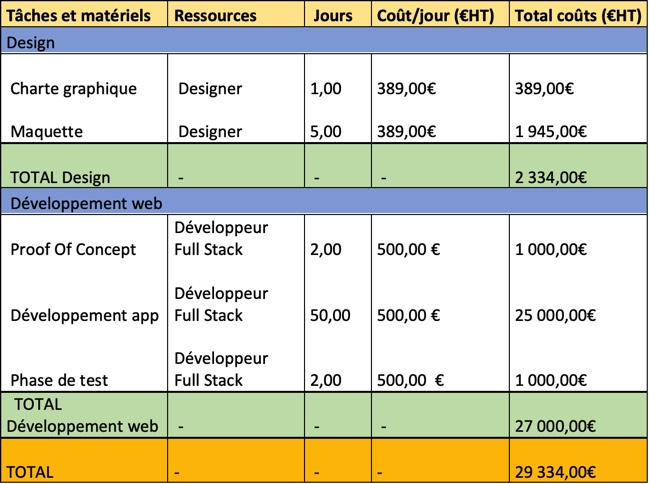
\includegraphics[scale=0.5]{img/estimation_prix_projetFL.jpeg}
    \caption{Tableau estimatif des coûts de développement de l'application finale}
    \label{fig:TabEstimationAppFL}
\end{figure}
\clearpage

Une autre option aurait été de travailler avec une entreprise de développeurs, ce qui permettra d’avoir un suivi régulier si des problèmes arrivent après le déploiement de la solution. Cette solution est bien évidemment plus onéreuse. On peut compter sur une moyenne de 800\euro~par jour pour chaque développeur. Cette option coûterait 45 534\euro~à Panorama Performance (voir ci-dessous Fig:  \ref{fig:TabEstimationAppDev}).


\begin{figure}[!h]
    \centering
    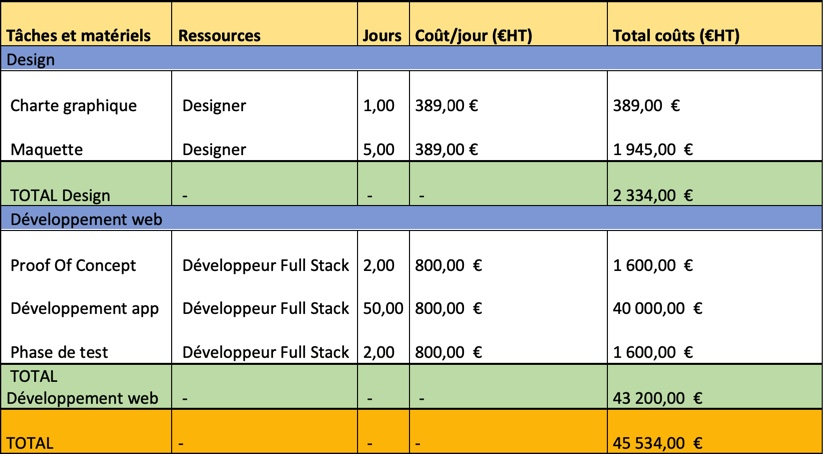
\includegraphics[scale=0.5]{img/estimation_prix_projetDev.jpeg}
    \caption{Tableau estimatif des coûts de développement de l'application finale par une entreprise de développement}
    \label{fig:TabEstimationAppDev}
\end{figure}


On peut donc en conclure que Panorama Performance sort gagnant de cette collaboration. En effet, ils auront, grâce à une somme dépensée de 2500\euro, bien inférieure à 10\% du coût final du projet, obtenu une version très poussée du séquenceur numérique ainsi qu’une étude de faisabilité de cette digitalisation.